\chapter{Artefakt-Design und Entwicklung}

Die Entwicklung des Artefakts folgte einem strukturierten Prozess, der sicherstellt, dass jede technische Entscheidung sowohl praxisnah als auch wissenschaftlich fundiert ist. In diesem Kapitel werden die Schritte zur Datenvorbereitung, Implementierung der Trainingspipeline und Hyperparameter-Optimierung detailliert diskutiert und begründet.

\section{Datensammlung und Analyse}

  Die vorliegende Arbeit nutzt Telemetriedaten aus der Porsche Motorsport Cloud Plattform. Es wurden sämtliche Rennsessions der \ac{IMSA}- und \ac{WEC}-Meisterschaften der Jahre 2023 bis 2025 extrahiert. Zur Minimierung von Varianz durch unterschiedliche Fahrsituationen beschränkt sich die Auswahl auf Rennsessions, während Trainings- und Qualifikationssessions ausgeschlossen wurden. Zusätzlich erfolgte eine Filterung auf Runden mit Trockenreifen, da Regenbedingungen weitere Einflussfaktoren einführen. Die Datenselektion wurde direkt beim Abruf mittels der ADX-\ac{KQL} vorgenommen, wodurch ein Rohdatensatz im CSV-Format mit 17 735 Runden (Datenpunkten) resultierte.

  Im Rahmen eines Experteninterviews mit dem Performance Engineer wurden jene Parameter identifiziert, die als Merkmale (Features) in das \ac{ML}-Modell eingehen.\footnote{Vgl. Experteninterview 2, 12.09.2025, Z. 37-53} Die Merkmale gliedern sich in kontinuierliche und kategoriale Features die in Tabelle-\ref{tab:features_channels} aufgelistet sind.

\begin{table}[H]
  \centering
  \footnotesize
  \begin{tabular}{|p{4cm}|p{4.5cm}|p{6cm}|}
    \hline
    \textbf{Feature Name} & \textbf{Channel Name} & \textbf{Erklärung} \\
    \hline
    \multicolumn{3}{|l|}{\textbf{Kontinuierliche Features}} \\
    \hline
    Umgebungstemperatur & TAmbientVms\_AVG & Lufttemperatur der Umgebung \\
    \hline
    Reifentemperatur VL & TTyreIRFLavg & Temperatur des vorderen linken Reifens (Innenrand) \\
    \hline
    Reifentemperatur VR & TTyreIRFRavg & Temperatur des vorderen rechten Reifens (Innenrand) \\
    \hline
    Reifentemperatur HL & TTyreIRRLavg & Temperatur des hinteren linken Reifens (Innenrand) \\
    \hline
    Reifentemperatur HR & TTyreIRRRavg & Temperatur des hinteren rechten Reifens (Innenrand) \\
    \hline
    Reifendruck VL & pTyreFL\_avg & Luftdruck des vorderen linken Reifens \\
    \hline
    Reifendruck VR & pTyreFR\_avg & Luftdruck des vorderen rechten Reifens \\
    \hline
    Reifendruck HL & pTyreRL\_avg & Luftdruck des hinteren linken Reifens \\
    \hline
    Reifendruck HR & pTyreRR\_avg & Luftdruck des hinteren rechten Reifens \\
    \hline
    Fuel Load & mFuelMass\_AVG & Aktuelle Kraftstoffmasse im Tank \\
    \hline
    Tyre Mileage VL & TyreMilage\_FL & Laufleistung des vorderen linken Reifens \\
    \hline
    Tyre Mileage VR & TyreMilage\_FR & Laufleistung des vorderen rechten Reifens \\
    \hline
    Tyre Mileage HL & TyreMilage\_RL & Laufleistung des hinteren linken Reifens \\
    \hline
    Tyre Mileage HR & TyreMilage\_RR & Laufleistung des hinteren rechten Reifens \\
    \hline
    Reifendruck Asymmetrie & tire\_pressure\_asymmetry & Asymmetrie zwischen linken und rechten Reifen \\
    \hline
    Reifendruck Balance & tire\_pressure\_balance & Balance zwischen Vorder- und Hinterachse \\
    \hline
    Reifendruck Spread & tire\_pressure\_spread & Spreizung der Reifendruckwerte \\
    \hline
    Reifen-Umgebungstemperatur Delta & tire\_temp\_ambient\_delta & Temperaturdifferenz Reifen zu Umgebung \\
    \hline
    Reifentemperatur Gradient Max & tire\_temp\_gradient\_max & Maximaler Temperaturgradient zwischen Reifen \\
    \hline
    \multicolumn{3}{|l|}{\textbf{Kategoriale Features}} \\
    \hline
    Mechanical Balance Front & NDriverARBSettingFAvg & Einstellung der vorderen Stabilisatorsteifigkeit \\
    \hline
    Mechanical Balance Rear & NDriverARBSettingRAvg & Einstellung der hinteren Stabilisatorsteifigkeit \\
    \hline
    Brake Balance & rBrakeBiasOffsetRequest\_AVG & Bremskraftverteilung Vorder-/Hinterachse \\
    \hline
    Traction Control Longitudinal & NTCLongitudinal\_AVG & Traktionskontrolle längs \\
    \hline
    Traction Control Lateral & NTCLateral\_AVG & Traktionskontrolle quer \\
    \hline
    Tyre State & NTyreState\_AVG & Reifenmischung(hart/medium/soft) \\
    \hline
    Event Category & eventCategory & Rennstrecke \\
    \hline
    \multicolumn{3}{|l|}{\textbf{Zielvariable}} \\
    \hline
    Understeer Average & aUndersteer\_AVG & Durchschnittlicher Untersteer-Wert pro Runde \\
    \hline
  \end{tabular}
  \caption{Übersicht der verwendeten Features und deren Channel-Namen}
  \label{tab:features_channels}
\end{table}

  Als Zielvariable dient der durchschnittliche Fahrzeugbalance-Wert pro Rennrunde (aUndersteer\_AVG), wobei Werte über Null Untersteuern und Werte unter Null Übersteuern des Fahrzeugs anzeigen. Dieser Wert wird in der Datenplattform bereits auf Basis physikalischer Formeln berechnet. Diese Berechnung wird aus Umfangsgründen nicht näher erläutert. Alle Parameter und die Zielvariable wurden rundenmittelnd aggregiert, sodass jeder Datensatzpunkt einer einzelnen Rennrunde entspricht.
  Die \ac{EDA} wurde durchgeführt, um die Dateneigenschaften zu untersuchen und potenzielle Datenqualitätsprobleme zu identifizieren. Zunächst wurde die Verteilung der Zielvariable aUndersteer\_AVG untersucht.\footnote{Vgl. \cite{Tukey1977}, S. 1–50}
\begin{figure}[H]
  \centering
  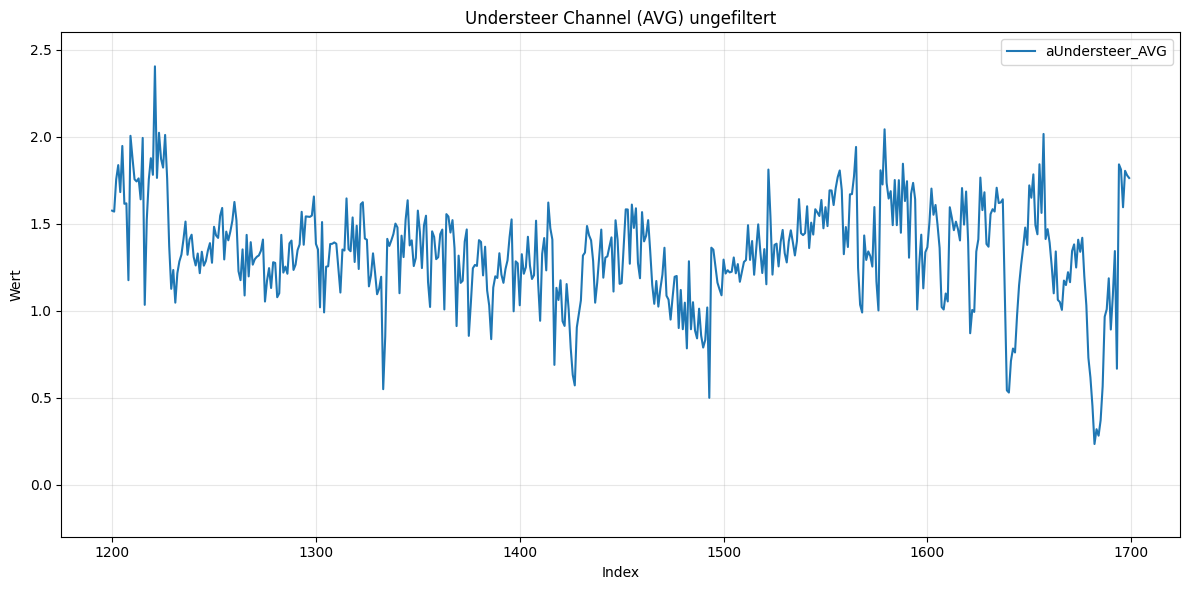
\includegraphics[width=0.8\textwidth]{graphics/understeer_nonfilt.png}
  \caption{Plot der Zielvariable aUndersteer\_AVG.}
  \label{fig:understeer_distribution}
\end{figure}
Der in Abbildung \ref{fig:understeer_distribution} dargestellte Verlauf des Fahrzeugbalance-Channels ist auffällig, denn obwohl es sich bereits um Durchschnitte über jeweils eine Runde handelt, weist der Graph eine hohe Volatilität auf.
Diese Erkenntnis sollte in der Modellierung der Vorverarbeitungsschritte berücksichtigt werden, um die Robustheit des Modells zu erhöhen.

Die Verteilungen der zentralen kontinuierlichen Features wurden ebenfalls untersucht. Abbildung \ref{fig:temp_distribution} zeigt exemplarisch die Verteilung der Reifentemperatur hinten-rechts. Dabei sind sowohl realistische, aber extreme Werte unter 40 Grad Celsius als auch auffällige, unrealistische Ausreißer über 300 Grad Celsius zu erkennen. Die Einschätzung, ob es sich um valide Daten handelt, erfolgt durch Informationen aus Experteninterviews.\footnote{Vgl. Experteninterview 1, 29.08.2025, Z. 97-105} Diese Ausreißer deuten auf potenzielle Sensorfehler oder Datenqualitätsprobleme hin und werden in der Datenvorbereitung entsprechend behandelt.
\begin{figure}[H]
  \centering
  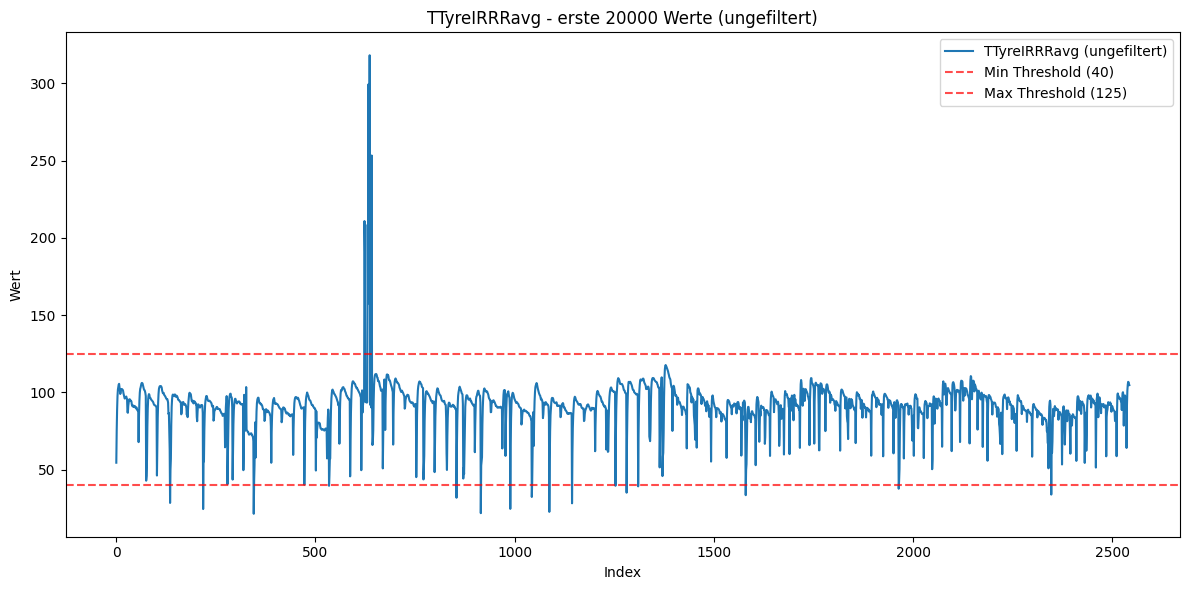
\includegraphics[width=0.8\textwidth]{graphics/TempPlot.png}
  \caption{Plot der Reifentemperatur hinten-rechts.}
  \label{fig:temp_distribution}
\end{figure}

Auch bei den Werten des Reifendrucks gibt es auffällige Ausreißer. Abbildung \ref{fig:druck_distribution} zeigt die Verteilung des Reifendrucks vorne-links. Hier sind ebenfalls unrealistische Werte zu erkennen, die auf mögliche Datenqualitätsprobleme hinweisen und in der Vorverarbeitung entsprechend berücksichtigt werden müssen.
\begin{figure}[H]
  \centering
  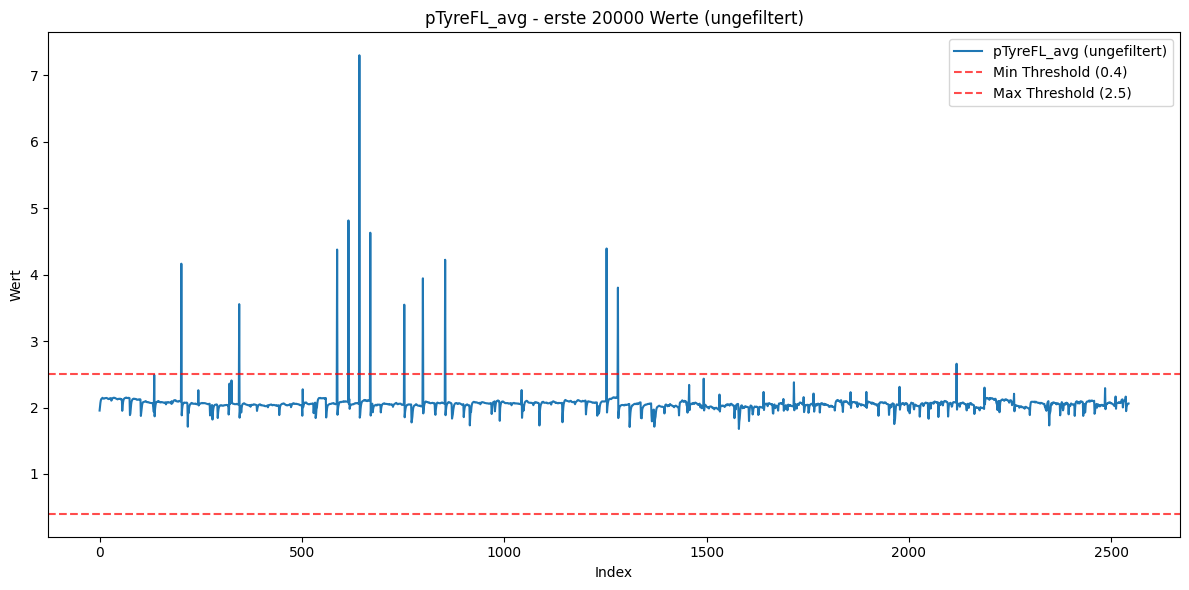
\includegraphics[width=0.8\textwidth]{graphics/DruckPlot.png}
  \caption{Plot des Reifendrucks vorne-links.}
  \label{fig:druck_distribution}
\end{figure}

Abschließend wurde mittels Korrelationsmatrix die Stärke der Zusammenhänge aller Merkmale untersucht. Dabei ergaben sich insbesondere enge Korrelationen zwischen den Reifentemperatur- und Reifendrucksensoren sowie zwischen der Kraftstoffmenge und der Anzahl der Runden pro Reifenlaufleistung. 
\begin{figure}[H]
  \centering
  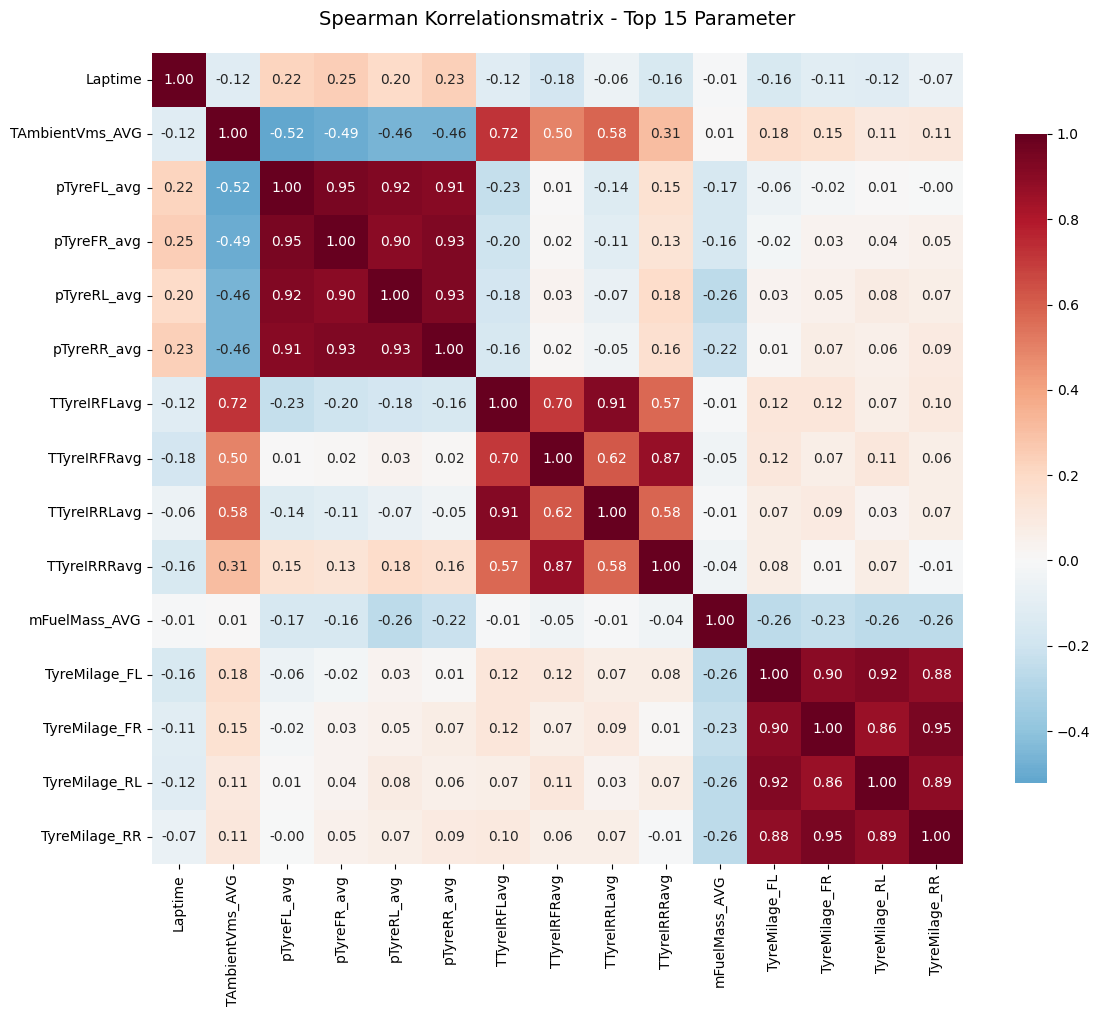
\includegraphics[width=0.8\textwidth]{graphics/korrelations_matrix_top.png}
  \caption{Korrelationsmatrix der 15 am stärksten korrelierten Parameter.}
  \label{fig:korrelations_matrix}
\end{figure}


Die explorative Analyse zeigte (i) stark schwankende Zielgrößen trotz Rundenglättung, (ii) häufige Ausreißer und Sensorartefakte bei Temperatur und Druck, sowie (iii) hohe Redundanzen in korrelierten Messkanälen (Reifen- und Drucksensorik, Fuel Load vs. Tyre Mileage). Im nächsten Abschnitt werden die daraus abgeleiteten Vorverarbeitungsschritte und das Feature-Engineering formalisiert und implementierungsorientiert beschrieben.



\section{Datenvorbereitung und Feature-Engineering}

Basierend auf den EDA-Erkenntnissen werden nachfolgend die systematischen Vorverarbeitungsschritte zur Transformation des Rohdatensatzes in ein trainingstaugliches Format dokumentiert.

\subsection{Ableitung der Vorverarbeitungsanforderungen}

Aus den Erkenntnissen der explorativen Datenanalyse ergeben sich konkrete Anforderungen an die Datenvorbereitung. Die hohe Volatilität der Zielvariable aUndersteer\_AVG erfordert Strategien zur Glättung von Zeitreihenschwankungen, da selbst rundenmittelnd aggregierte Werte eine unregelmäßige Verteilung aufweisen. Die identifizierten Sensorartefakte bei Reifentemperaturen über 300 Grad Celsius und unrealistische Werte bei Reifendruckmessungen indizieren Messfehler, die durch domänenbasierte Schwellwertfilterung adressiert werden müssen.\footnote{Vgl. Experteninterview 2, 12.09.2025, Z. 42-53} Ferner zeigt die Korrelationsmatrix aus Abschnitt 4.1 starke Abhängigkeiten zwischen einzelnen Sensoren derselben physikalischen Größe, was eine Reduktion redundanter Features nahelegt. \footnote{Vgl. \cite{Guyon2003}, S. 1165–1170}


Diese Anforderungen entsprechen den Design Requirements für das Datenartefakt im Sinne der \ac{DSR}-Methodik. Die Vorverarbeitungsentscheidungen werden transparent dokumentiert und auf drei Quellen zurückgeführt: (i) datengetriebene Erkenntnisse der EDA, (ii) domänengetriebene Validierung durch Experteninterviews sowie (iii) theoriegetriebene Fundierung durch etablierte \ac{ML}-Literatur zu Datenvorverarbeitung und Ausreißererkennung.


\subsection{Datenbereinigung und Filterung}

Zur Minimierung systematischer Verzerrungen wurden zunächst alle Out-Laps (Runde = 1) aus dem Datensatz entfernt. Out-Laps weisen typischerweise atypische Charakteristika auf, da Fahrzeuge die Boxengasse verlassen und sich das thermische Verhalten der Reifen von regulären Rennrunden unterscheidet. Diese Filterregel reduziert Varianz durch nicht-repräsentative Datenpunkte und stellt sicher, dass das Modell ausschließlich auf Basis von Rennrunden mit stabilisiertem Fahrzeugverhalten trainiert wird.

Eine weitere Quelle von Varianz sind Extremereignisse während des Rennens, wie Unfälle, Safety-Car-Phasen oder technische Defekte. Diese manifestieren sich in der Regel durch extreme Abweichungen der Rundenzeit vom durchschnittlichen Niveau. Zur Identifikation solcher Ereignisse wurde eine statistische Schwellwertmethode angewendet. Runden, deren Rundenzeit um mehr als eine Standardabweichung (ca. 40 Sekunden) vom Mittelwert abweichen, wurden aus dem Datensatz entfernt. Diese Filterung folgt etablierten statistischen Verfahren zur Ausreißererkennung in Zeitreihendaten und trägt zur weiteren Varianzreduktion bei.\footnote{Vgl. \cite{Box2015}, S. 408–450}

Für die kontinuierlichen Features Reifentemperatur und Reifendruck wurden domänenspezifische Schwellwerte zur Erkennung und Entfernung unrealistischer Messwerte definiert. Wie in Abbildung \ref{fig:temp_distribution} dargestellt, treten bei Reifentemperaturen Werte über 300 Grad Celsius auf, die physikalisch nicht plausibel sind und auf Sensorfehler hindeuten. Analog zeigen Reifendruckmessungen (Abbildung \ref{fig:druck_distribution}) Ausreißer außerhalb realistischer Bereiche. 
Die Festlegung der konkreten Grenzwerte erfolgte unter Einbeziehung von Expertenwissen.\footnote{Vgl. Experteninterview 1, 29.08.2025, Z. 97-105} 
Dieser domänenbasierte Ansatz zur Ausreißererkennung ist in der \ac{ML}-Literatur als effektive Methode etabliert, wenn technisches Fachwissen verfügbar ist.\footnote{Vgl. \cite{Kuhn2019}, S. 73–75} Die Implementierung erfolgte durch Filterregeln, die Datenpunkte außerhalb der definierten Grenzwerte ausschließen.

\begin{table}[H]
  \centering
  \begin{tabular}{lcc}
    \toprule
    \textbf{Feature-Kategorie} & \textbf{Unterer Grenzwert} & \textbf{Oberer Grenzwert} \\
    \midrule
    Reifendruck (alle Räder) [bar] & 1,3 & 2,5 \\
    Reifentemperatur (alle Räder) [°C] & 40 & 125 \\
    Kraftstoffmasse [kg] & 0 & 120 \\
    \bottomrule
  \end{tabular}
  \caption{Domänenbasierte Schwellwerte für Ausreißererkennung}
  \label{tab:threshold_values}
\end{table}


\subsection{Feature-Engineering und Dimensionsreduktion}

Die in Abschnitt 4.1 präsentierte Korrelationsmatrix (Abbildung \ref{fig:korrelations_matrix}) offenbart hohe Korrelationen zwischen einzelnen Sensoren der Reifentemperatur sowie des Reifendrucks. Solche redundanten Features können bei \ac{ML}-Modellen zu Multikollinearität führen und die Interpretierbarkeit reduzieren. Multikollinearität bezeichnet dabei die starke lineare Abhängigkeit zwischen zwei oder mehr unabhängigen Variablen, wodurch deren individuelle Einflussnahme auf die Zielvariable im Modell schwer zu unterscheiden ist. \footnote{Vgl. \cite{James2021}, S. 107–110; vgl. dazu auch \cite{Guyon2003}, S. 1165-1170; vgl. dazu auch \cite{YuLiu2004}, S. 1205-1224} 
Zur Quantifizierung der Redundanz wurde ein korrelationsbasiertes Verfahren angewendet: Features mit einer absoluten Pearson-Korrelation über 0,9 zu anderen Features wurden als hochkorreliert klassifiziert.\footnote{Vgl. \cite{Kuhn2019}, S. 180-190; vgl. dazu auch \cite{Hall1999}, S. 51-103} Die Identifikation dieser Feature-Gruppen bildet die Grundlage für die nachfolgende Feature-Aggregation.
Anstatt hochkorrelierte Features vollständig zu entfernen, wurden neue motorsport-relevante Features durch statistische Zusammenfassung der Sensorgruppen erstellt. Aus den vier Reifendruck-Sensoren (vorne-links, vorne-rechts, hinten-links, hinten-rechts) und den entsprechenden Temperatursensoren wurden folgende abgeleitete Features generiert:

\begin{itemize}
  \item \textbf{tire\_pressure\_asymmetry}: Links-Rechts-Balance (|FL - RL|)
  \item \textbf{tire\_pressure\_balance}: Vorn-Hinten-Balance (Durchschnitt vorne - hinten)
  \item \textbf{tire\_pressure\_spread}: Setup-Homogenität (max - min aller Drücke)
  \item \textbf{tire\_temp\_ambient\_delta}: Arbeitstemperatur relativ zur Umgebung
  \item \textbf{tire\_temp\_gradient\_max}: Maximales thermisches Ungleichgewicht (max - min Temperaturen)
\end{itemize} Diese Transformation reduziert die Dimensionalität bei gleichzeitigem Erhalt der relevanten Information und kann die Modellgeneralisierung verbessern.\footnote{Vgl. \cite{Guyon2003}, S. 1158–1161}
Um die Auswirkung dieser Dimensionsreduktion auf die Modellperformance empirisch zu evaluieren, wurden zwei Feature-Konfigurationen erstellt: (i) Datensätze mit aggregierten Features bei gleichzeitigem Entfernen der hochkorrelierten Original-Features sowie (ii) Datensätze mit aggregierten Features bei Beibehaltung aller Original-Features. Diese experimentelle Designentscheidung ermöglicht eine systematische Bewertung des Trade-offs zwischen Dimensionalität und Informationsgehalt in der späteren Evaluationsphase.

Der Datensatz enthält zudem kategoriale Features wie die Tracktionskontroll-Settings und weitere diskrete Variablen (siehe Tabelle \ref{tab:features_channels}). Für die Track-Variable wurde eine ordinale Kodierung vorgenommen: Die alphabetisch sortierten Streckennamen wurden numerischen Codes zugeordnet (TrackCode). Diese Zuordnung wurde in einer separaten Mapping-Datei dokumentiert, um die Rückverfolgbarkeit zu gewährleisten und eine konsistente Kodierung zwischen Trainings- und Validierungsdaten sicherzustellen.\footnote{Vgl. \cite{Chen2016}, S. 786–787}
Eine One-Hot-Encodierung kategorialer Features wurde bewusst nicht durchgeführt, da die in dieser Arbeit verwendeten baumbasierten Modelle XGBoost und LightGBM kategoriale Features, welche im nächsten Abschnitt genau behandelt werden, nativ unterstützen.\footnote{Vgl. \cite{Chen2016}, S. 786–788; vgl. dazu auch \cite{Ke2017}, S. 1-10} Diese Algorithmen implementieren spezialisierte Split-Strategien für kategoriale Variablen, die gegenüber One-Hot-Encodierung Vorteile in Bezug auf Speichereffizienz und Modellperformance bieten.\footnote{Vgl. \cite{Chen2016}, S. 787-789}
Zur Untersuchung des Einflusses kategorialer Features auf die Modellleistung wurden zusätzlich Datensatzvarianten ohne kategoriale Features erstellt. Diese Designentscheidung folgt dem Prinzip der systematischen Evaluation multipler Artefaktvarianten in der Build-Phase der \ac{DSR}-Methodik.


\subsection{Zielvariablen-Glättung}

Trotz der rundenmittelnd aggregierten Zielvariable aUndersteer\_AVG zeigt deren zeitlicher Verlauf (Abbildung \ref{fig:understeer_distribution}) eine hohe Volatilität. Diese kurzfristigen Schwankungen können durch situative Faktoren wie Verkehrssituationen, Überholmanöver oder kurzzeitige Setup-Änderungen verursacht werden und erschweren die Identifikation längerfristiger Trends im Fahrzeugverhalten.
Zur Adressierung dieser Problematik wurde eine Glättungsstrategie mittels gleitender Durchschnitte (Moving Averages) implementiert. Gleitende Durchschnitte sind eine etablierte Methode zur Rauschreduktion in Zeitreihendaten und werden häufig im Feature Engineering eingesetzt.\footnote{Vgl. \cite{Box2015}, S. 25-40} Die Methode berechnet für jede Runde den Durchschnitt über ein Fenster von $n$ benachbarten Runden, wodurch kurzfristige Fluktuationen gedämpft werden.
Um die optimale Fenstergröße zu ermitteln, wurden mehrere Glättungsvarianten mit unterschiedlichen Fenstergrößen erstellt: keine Glättung (Baseline), sowie gleitende Durchschnitte mit Fenstergrößen 2, 3 und 4.
Die Wahl dieser Fenstergrößen basiert auf folgender Überlegung: Kleinere Fenster (2, 3) erfassen kurzfristige Schwankungen und erhalten mehr Details, während größere Fenster (4) stärker glätten und langfristigere Trends betonen.\footnote{Vgl. \cite{Box2015}, S. 35-45} Die ungeglättete Variante dient als Referenz zur Quantifizierung des Effekts der Glättung auf die Modellperformance.
Diese multiplen Glättungsvarianten stellen alternative Designentscheidungen dar, die im Rahmen der iterativen Build-Evaluate-Phasen der \ac{DSR}-Methodik systematisch evaluiert werden. Die Erstellung mehrerer Varianten ermöglicht eine empirische Bewertung des Trade-offs zwischen Rauschreduktion und Informationsverlust.


\subsection{Datensatz-Aufteilung und Validierungsstrategie}

Die Kombination der beschriebenen Vorverarbeitungsoptionen resultiert in einer systematischen Variation von Datensatzkonfigurationen. Die Designentscheidungen umfassen drei Dimensionen:

\begin{enumerate}
  \item \textbf{Kategoriale Features:} mit kategorialen Features vs. ohne kategoriale Features (2 Varianten)
  \item \textbf{Feature-Reduktion:} aggregierte Features mit Entfernung hochkorrelierter Original-\\Features vs. aggregierte Features zusätzlich zu Original-Features (2 Varianten)
  \item \textbf{Zielvariablen-Glättung:} keine Glättung, Fenstergröße 2, 3, 4 (4 Varianten)
\end{enumerate}
Die vollständige Kombination dieser Dimensionen ergibt $2 \times 2 \times 4 = 16$ Trainingsdatensätze. Jeder Datensatz umfasst nach Anwendung aller Filterungsschritte ca. 9\,000 Runden (Datenpunkte).

Die Validierung der entwickelten Modelle erfordert separate Validierungsdatensätze, die während des Trainings nicht zugänglich sind. Um die Generalisierungsfähigkeit der Modelle umfassend zu bewerten, wurden zwei komplementäre Validierungsstrategien implementiert:

\textbf{Event-basierte Validierung (Leave-One-Out):}
Ein vollständiges Renn-Event wurde vom Trainingsdatensatz separiert und als Validierungsdatensatz reserviert. Diese Strategie prüft die Fähigkeit des Modells, auf eine neue, ungesehene Kombination von Strecke, Wetterbedingungen und Rennsituation zu generalisieren.\footnote{Vgl. \cite{James2021}, S. 185-193} Der Event-Validierungsdatensatz umfasst ca. 200 Runden.

\textbf{Zufällige Validierung:}
Aus dem verbleibenden Datensatz wurden 10\,\% der Runden zufällig ausgewählt und als zweiter Validierungsdatensatz verwendet. Diese Strategie entspricht der etablierten Praxis des Train-Test-Splits in der \ac{ML}-Literatur und dient der Bewertung der Modellperformance auf typischen, aber ungesehenen Datenpunkten.\footnote{Vgl. \cite{James2021}, S. 32-35} Der Zufalls-Validierungsdatensatz umfasst ca. 1\,000 Runden.

Für beide Validierungsstrategien wurden Datensätze entsprechend der zwei Feature-\\Konfigurationen (mit/ohne kategoriale Features) und der zwei Reduktionsstrategien (mit/ohne Entfernung hochkorrelierter Features) erstellt. Dies resultiert in $2 \times 2 \times 2 = 8$ Validierungsdatensätzen.
Die zweifache Validierungsstrategie ermöglicht eine differenzierte Robustheitsbewertung: Die Event-basierte Validierung testet die Extrapolationsfähigkeit auf vollständig neue Kontexte, während die zufällige Validierung die Interpolationsfähigkeit innerhalb der Verteilung der Trainingsdaten bewertet. Diese Kombination entspricht best practices im \ac{ML} und erhöht die Aussagekraft der Modellbewertung.\footnote{Vgl. \cite{James2021}, S. 175-201}


\subsection{Technische Implementierung}

Die beschriebenen Vorverarbeitungsschritte wurden in einem Python-Skript implementiert. Die Pipeline verarbeitet die Rohdaten (17\,735 Runden aus der KQL-Extraktion) in einer klar definierten Sequenz: Zunächst werden die Daten eingelesen und unmittelbar um nicht-repräsentative Out-Laps sowie extrem abweichende Rundenzeiten bereinigt. Anschließend entfernt eine domänenbasierte Schwellwertlogik physikalisch unrealistische Sensorwerte. Darauf folgt das Feature-Engineering, in dessen Rahmen hochkorrelierte Sensorkanäle durch aggregierte, informationsverdichtete Kennwerte ersetzt bzw. ergänzt und kategoriale Merkmale ordinal kodiert werden. Im nächsten Schritt erzeugt die Pipeline alternative Zielvarianten durch optionale Glättung (keine, Fenster 2, 3, 4), wodurch parallele Datensatzkonfigurationen für die spätere Modellselektion entstehen. Abschließend werden zwei Validierungsperspektiven vorbereitet: ein vollständig herausgelöstes Renn-Event (Extrapolation) sowie ein zufälliger Anteil von 10 \% der verbleibenden Runden (Interpolation). Aus der vollständigen Kreuzung der Vorverarbeitungsoptionen resultieren so 16 Trainingsdatensätze und 8 korrespondierende Validierungsdatensätze, die konsistent im CSV-Format versioniert abgelegt werden.

Die Implementierung stellt Reproduzierbarkeit durch konsistente Transformation aller Datensatzvarianten sicher. Alle Mapping-Dateien und Konfigurationsparameter wurden dokumentiert und versioniert.

Im Kontext der \ac{DSR}-Methodik stellt dieses Kapitel die Build-Phase der Datenpipeline dar. Die multiplen Datensatzvarianten ermöglichen eine systematische Evaluation der Auswirkungen unterschiedlicher Vorverarbeitungsentscheidungen auf die Modellperformance in der nachfolgenden Evaluate-Phase. Die transparente Dokumentation aller Designentscheidungen mit Rückführung auf EDA-Erkenntnisse, Expertenwissen und theoretische Fundierung erfüllt die Rigor-Anforderungen der \ac{DSR}-Methodik.
Die vorbereiteten Datensätze bilden die Grundlage für die Modellentwicklung und Hyperparameter-Optimierung im nachfolgenden Abschnitt 4.3.



\section{Modelltraining und Hyperparameter-Optimierung}

Die Modelltrainingsphase bildet den Kern der Artefakt-Entwicklung und zielt darauf ab, aus den in Abschnitt 4.2 generierten 16 Datensatzstrukturen robuste Vorhersagemodelle abzuleiten. Hierzu werden zwei Gradient-Boosting-Algorithmen – XGBoost und LightGBM – auf vier abgestuften Komplexitätsniveaus mittels systematischer Hyperparameter-Optimierung trainiert und anschließend auf strukturkonsistenten Validierungsdatensätzen evaluiert.

Neben \ac{GBDT} wurden lineare Modelle (Linear, Ridge, Lasso), \ac{SVR}, Random Forest sowie Deep-Learning-Architekturen (MLP, TabNet) als Alternativen geprüft. Lineare Ansätze erfassen komplexe nichtlineare Zusammenhänge der Telemetriedaten nur begrenzt, \ac{SVR} skaliert bei \(~9\,000\) Runden und fehlender nativer Unterstützung kategorialer Merkmale ungünstig.\footnote{Vgl. \cite{Pasaribu2024}, S. 3–4} Random Forest liefert zwar robuste Baselines, erreicht aber in tabularen Regressionen häufig nicht die Spitzengenauigkeit moderner Boosting-Methoden.\footnote{Vgl. \cite{Geeks2024}, S. 4–6; vgl. dazu auch \cite{Hastie2009}, S. 587–590} Neuronale Netze zeigen auf mittelgroßen tabularen Datensätzen gegenüber fortgeschrittenem Baum-Boosting Performance-Nachteile.\footnote{Vgl. \cite{McElfresh2023}, S. 1–3} Aus diesen Gründen fokussiert sich das Artefakt auf Gradient-Boosting-Entscheidungsbäume als günstigen Kompromiss aus Prognosegüte, Interpretierbarkeit und Umsetzbarkeit.
Zwei komplementäre Implementierungen desselben Paradigmas werden eingesetzt: XGBoost für Regularisierung und Stabilität, LightGBM für Effizienz und Trainingsgeschwindigkeit. Beide können kategoriale Merkmale direkt verarbeiten und reduzieren so Kodierungsaufwand und Komplexität.\footnote{Vgl. \cite{Chen2016}, S. 786-791; vgl dazu auch \cite{Ke2017}, S. 3157–3168} Die Parallelnutzung folgt dem \ac{DSR}-Prinzip vergleichender Evaluation theoretisch fundierter Artefakt-Alternativen.

Die Trainingspipeline führt für jede der 16 Datensatzstrukturen denselben reproduzierbaren Ablauf aus: (i) Einlesen und Aufteilung in Features/Zielvariable, (ii) systematische Hyperparameter-Suche mittels dreifacher Kreuzvalidierung, (iii) Retraining des besten Konfigurationsprofils auf allen Trainingsdaten zur Maximierung der Vorhersagequalität, (iv) strukturierte Persistierung von Modell, Parametern und Metriken (R², RMSE, MAE). Deterministische Zufallssaaten und parallele Ausführung (scikit-learn-kompatible API) gewährleisten Vergleichbarkeit und Reproduzierbarkeit.\footnote{Vgl. \cite{Pedregosa2011}, S. 2825–2830}

Für die Hyperparameter-Optimierung wird \texttt{GridSearchCV} eingesetzt: exhaustive Suche über klar abgegrenzte Parameter-Intervalle, primäre Bewertungsmetrik ist $R^2$ (direkt interpretierbar für Fachexperten), ergänzt durch Fehlermaße zur Einschätzung der Abweichungsgrößenordnung.\footnote{Vgl. \cite{Bergstra2012}, S. 281–305; vgl. dazu auch \cite{Pedregosa2011}, S. 2828–2829} Die dreifache Kreuzvalidierung bietet robuste Schätzungen bei vertretbarem Aufwand.

Abgestufte Komplexitätsprofile strukturieren die Suche:
\begin{description}
  \item[Shallow:] $n\_estimators$: 50–100, $\max\_depth$: 3–4, $\eta$: 0.1–0.2.
  \item[Medium:] $n\_estimators$: 100–500, $\max\_depth$: 5–9, $\eta$: 0.05–0.1.
  \item[Deep:] $n\_estimators$: 300–700, $\max\_depth$: 10–12, $\eta$: 0.03–0.05.
  \item[Very Deep:] $n\_estimators$: 400–800, $\max\_depth$: 10–15, $\eta$: 0.02–0.03.
\end{description}
Zusätzlich variieren \texttt{subsample} (0.8/1.0), \texttt{colsample\_bytree} (0.8/1.0) bzw. \texttt{feature\_fraction}, \texttt{min\_child\_weight}/\texttt{min\_child\_samples}.

Beide Verfahren haben das Ziel, eine quadratische Fehlerfunktion zu minimieren.\footnote{Vgl. \cite{Chen2016} S. 786-787; vgl. dazu auch \cite{Ke2017}, S. 1-10} L2 ist konsistent mit $R^2$, da eine Reduktion der Residuen direkt zu höherer Erklärungsvarianz führt. Gewählt wurde L2 aufgrund (i) Etabliertheit in tabularer Regression, (ii) stabiler Optimierungseigenschaften (glatte Gradienten), (iii) direkter Interpretierbarkeit ergänzender Fehlerkennzahlen (RMSE/MAE). Alternativen wie Huber- oder Quantile-Loss wurden nicht priorisiert, weil potenzielle Ausreißer bereits vorab bereinigt wurden und zusätzliche Komplexität ohne klaren Mehrwert vermieden wird.

Aus der Kreuzung von 16 Datensatzstrukturen, zwei Boosting-Implementierungen und vier Komplexitätsstufen entstehen \textbf{128 trainierte Modelle}.







\section{Validierung und Modellvergleich}
\label{sec:validierung_modellvergleich}

Die abschließende Validierung erfolgt in einem dedizierten Jupyter-Notebook, das die finalen Modelle auf einem zuvor ungesehenen Validierungsdatensatz evaluiert und vergleichbar macht.
Dafür wird jedes Modell einzeln geladen und auf beiden Datensätzen (Event und Zufalls-Datensatz) evaluiert. Das Ergebnis sind insgesamt \textbf{256 Evaluationsergebnisse} die aus den Evaluationsmetriken $R^2$, RMSE und MAE, für jedes Modell bestehen.
\noindent
Dadurch wird transparent, welche Modelltyp-/Feature-Kombination auf neuen, ungesehenen Telemetriedaten am besten generalisiert. 
